\documentclass{article}
\usepackage[utf8]{inputenc}
\usepackage{graphicx}
\usepackage{amsmath}
\usepackage{subcaption}
\usepackage{listings}
\usepackage{minted}
\usepackage{booktabs}
\usepackage[a4paper, total={6in, 9in}]{geometry}

\title{Sparse Square Matrix Multiplication using MPI}
\author{
  Biwei Tang, Yunxiang Yan, Qidian Gao \\
  Department of Computer Science and Engineering \\
  CS 6220 Project Assignment 3\\
  Georgia Institute of Technology
}
\date{April 2024}

\begin{document}

\maketitle

\begin{abstract}
    This report details the implementation and analysis of parallel sparse matrix multiplication. We focus on the effectiveness of using MPI for handling sparse matrices represented as arrays of tuples. Performance metrics are provided for different matrix sizes and sparsity parameters, demonstrating both strong scaling and the impact of sparsity on computational efficiency.
\end{abstract}

\section{Introduction}

This assignment for CX 4220/CSE 6220 Introduction to High Performance Computing for Spring 2024, Programming Assignment 3, addresses the efficient parallel multiplication of sparse matrices using MPI. Sparse matrices, predominantly filled with zeros, provide a unique challenge distinct from their dense counterparts. George P. Brudell's approach, storing matrices as arrays of (row, col, value) tuples, optimizes space but complicates multiplication.

The objective is to devise a parallel algorithm that multiplies two large square sparse matrices efficiently, with performance measured against the number of non-zero elements. Implementing this using MPI involves leveraging parallel processing to enhance computation speeds significantly.

Key requirements include:
\begin{itemize}
    \item \textbf{Sparse Matrix Representation:} Using a tuple array format, matrices A and B are generated with a random number generator that assigns non-zero values based on a specified sparsity parameter.
    \item \textbf{Efficient Parallel Computation:} The algorithm aims to surpass traditional dense matrix multiplication efficiencies through strategic data transfers and effective MPI utilization.
    \item \textbf{Matrix Operations:} Matrix B is transposed using MPI's Alltoallv, allowing for optimized multiplication within a ring topology, facilitating necessary dot products for the resultant matrix C.
    \item \textbf{Output in Dense Format:} While inputs maintain a sparse format, the resulting matrix C is outputted in a dense 2D array format, segmented across processors.
\end{itemize}

Our implementation introduces optimized data structures and computational techniques that significantly reduce the processing time for large matrix sizes and various sparsity levels. We employ advanced MPI features to improve data handling and matrix operations, emphasizing the strong scaling of our approach.

Experimental evaluation is conducted to compare theoretical predictions with actual performance, providing insights into the effectiveness of our parallel strategies in handling large-scale sparse matrix operations efficiently.

\textbf{Note:} All project details, including implementation strategies and experimental results, are confidential and should not be disclosed publicly to uphold academic integrity.


\section{Algorithm Description}
\subsection{Generating Sparse Matrix}
The sparse matrix is generated using the function \texttt{generateSparseMatrix}. Each element of the matrix is determined randomly based on a given sparsity factor. The matrix is distributed among the processes, where each process generates its portion of the matrix.

\begin{minted}[frame=lines, framesep=2mm, baselinestretch=1.2, fontsize=\footnotesize, linenos]{cpp}
    mt19937_64 gen(seed);
    uniform_real_distribution<> dis(0.0, 1.0);
    vector<SparseElement> matrix;
    uniform_int_distribution<uint64_t> val_dis(1, (1ull << 31) - 1);
    int rows_per_proc = n / p;
    for (int i = 0; i < rows_per_proc; ++i) {
        for (int j = 0; j < n; ++j) {
            if (dis(gen) < s) {
                matrix.push_back(make_tuple(i + r * rows_per_proc, j, val_dis(gen)));
            }
        }
    }
    return matrix;
}
\end{minted}

\subsection{Matrix Transposition Using MPI}
The transposition of matrix B is essential for the multiplication. This is done using the MPI function \texttt{MPI\_Alltoallv} to redistribute the matrix elements according to their transposed positions across all processes.

\begin{minted}[frame=lines, framesep=2mm, baselinestretch=1.2, fontsize=\footnotesize, linenos]{cpp}
void transposeMatrixB(const vector<SparseElement>& localB, int n,
vector<SparseElement>& localTransposedB, MPI_Comm comm) {
    int size, rank;
    MPI_Comm_size(comm, &size);
    MPI_Comm_rank(comm, &rank);
    int cols_per_proc = n / size;
    vector<int> send_counts(size, 0);
    vector<vector<SparseElement>> send_buffers(size);
    for (const auto& elem : localB) {
        int col_owner = get<1>(elem) / cols_per_proc;
        send_buffers[col_owner].push_back(elem);
        send_counts[col_owner]++;
    }
    vector<SparseElement> flat_send_buffer;
    vector<int> sdispls(size, 0);
    for (int i = 0; i < size; ++i) {
        sdispls[i] = flat_send_buffer.size();
        flat_send_buffer.insert(flat_send_buffer.end(), send_buffers[i].begin(), send_buffers[i].end());
    }
    vector<int> recv_counts(size);
    MPI_Alltoall(send_counts.data(), 1, MPI_INT, recv_counts.data(), 1, MPI_INT, comm);
    vector<int> rdispls(size, 0);
    for (int i = 1; i < size; ++i) {
        rdispls[i] = rdispls[i - 1] + recv_counts[i - 1];
    }
    int total_recv = rdispls[size - 1] + recv_counts[size - 1];
    vector<SparseElement> recv_buffer(total_recv);
    for (int i = 0; i < size; i++) {
        send_counts[i] *= sizeof(SparseElement);
        sdispls[i] *= sizeof(SparseElement);
        recv_counts[i] *= sizeof(SparseElement);
        rdispls[i] *= sizeof(SparseElement);
    }
    MPI_Alltoallv(flat_send_buffer.data(), send_counts.data(), sdispls.data(), MPI_BYTE,
                  recv_buffer.data(), recv_counts.data(), rdispls.data(), MPI_BYTE, comm);
    localTransposedB = std::move(recv_buffer);
}
\end{minted}

\subsection{Sparse Matrix Multiplication}
The core of the algorithm is the multiplication of sparse matrices. This function performs the dot product between matching elements of matrix A and the transposed matrix B, which have been distributed across the processors.

\begin{minted}[frame=lines, framesep=2mm, baselinestretch=1.2, fontsize=\footnotesize, linenos]{cpp}
void multiplySparseMatrices(const vector<SparseElement>& A,
const vector<SparseElement>& transposedB, int n, int size, vector<vector<uint64_t>>& localC) {
    int rows_per_proc = n / size;
    for (const auto& a : A) {
        int aRow = get<0>(a) % rows_per_proc;
        int aCol = get<1>(a);
        uint64_t aValue = get<2>(a);
        for (const auto& b : transposedB) {
            if (aCol == get<0>(b)) {
                int bCol = get<1>(b);
                uint64_t bValue = get<2>(b);
                localC[aRow][bCol] += aValue * bValue;
            }
        }
    }
}
\end{minted}

\section{Algorithm Complexity Analysis}

\subsection{Generating Sparse Matrix}

\subsubsection{Time Complexity}
The time complexity for generating a sparse matrix is dictated by the total operations required to iterate through each possible matrix element and conditionally add it to the matrix based on the sparsity factor \( s \). For a matrix of size \( n \times n \) distributed across \( p \) processors, each processor is responsible for approximately \( n^2 / p \) elements, resulting in an average number of operations of \( n^2 / p \times s \).

\subsubsection{Space Complexity}
The space complexity is determined by the storage required for the non-zero elements of the matrix. Given that the sparsity \( s \) dictates the fraction of non-zero elements, the expected storage requirement per processor is approximately \( n^2 / p \times s \) elements, where each element is represented by a tuple containing two integers and a numerical value.

\subsection{Matrix Transposition Using MPI}

\subsubsection{Time Complexity}
The time complexity of the matrix transposition phase involves iterating over the local matrix elements to classify and buffer them for redistribution. This operation is \( O(n^2 / p \times s) \). The redistribution itself, performed by \texttt{MPI\_Alltoallv}, typically involves a complexity of \( O(p + m) \), where \( m \) is the total number of elements being communicated, proportional to \( n^2 \times s \).

\subsubsection{Space Complexity}
Space complexity includes the need for local storage of matrix segments and additional buffers for the transposition process. Each processor may need to allocate space for up to \( n^2 \times s \) elements collectively across the send and receive buffers during the peak of the transposition operation.

\subsection{Sparse Matrix Multiplication}

\subsubsection{Time Complexity}
Each processor computes the product of local segments of matrices A and B. Assuming each processor holds \( n^2 / p \times s \) elements of A and B, the worst-case time complexity can reach \( O((n^2 / p \times s)^2) \) when each element of A is matched against elements in B. However, given the sparsity, the practical complexity is expected to be much lower.

\subsubsection{Space Complexity}
The space complexity is mainly influenced by the storage of the local segments of A and B, plus the result matrix C. Assuming C stores a result for every matrix element (if C is considered dense), each processor might need to handle \( n^2 / p \) elements for C, plus the sparse storage for A and B.

\section{Experimental Results}
\subsection{Setup}
Experiments were conducted on the PACE ICE cluster with up to 16 processors. Matrix sizes of 2000, 5000, and 10000 were tested with sparsity parameters of 0.1, 0.01, and 0.001. The test file we use is:

\begin{minted}[frame=lines, framesep=2mm, baselinestretch=1.2, fontsize=\footnotesize, linenos]{cpp}
#!/bin/bash

# Unload any conflicting MPI modules
module unload mvapich2/2.3.6-ouywal
# Load the required OpenMPI module
module load openmpi/4.1.4

# Configure the output file
output_file="experiment_results.txt"
echo "Running experiments for fixed sparsity e=0.01 with different matrix sizes" > $output_file

for n in 2000 4000 8000
do
    echo "Running size $n with 16 processors" >> $output_file
    mpirun -np 16 ./spmat $n 0.01 1 output_$n.txt >> $output_file 2>&1
done

echo "Running experiments for fixed matrix size n=10000 with varying sparsity" >> $output_file
for e in 0.1 0.01 0.001
do
    for p in 2 4 8 16
    do
        echo "Running sparsity $e with $p processors" >> $output_file
        mpirun -np $p ./spmat 10000 $e 1 output_n10000_e${e}_p${p}.txt >> $output_file 2>&1
    done
done

echo "All experiments completed." >> $output_file

\end{minted}

\subsection{Results}
We employed \textbf{O3} in \textbf{Makefile} to boost compile efficiency, and test-ran multiple times on \textbf{PACE ICE Cluster}. While it successfully generated output, we recorded the runtime:
\begin{table}[H]
\centering
\begin{tabular}{cc}
\toprule
\( p = 16 \) & \( e = 0.01 \) \\
\midrule
\( n = 2000 \) & 0.091643 \\
\( n = 4000 \) & 0.530882 \\
\( n = 8000 \) & 3.306465 \\
\bottomrule
\end{tabular}
\caption{Running times for matrix sizes of 2000, 4000, and 8000 with \( p = 16 \) processors and sparsity \( e = 0.01 \).}
\label{tab:table1}
\end{table}
\begin{table}[ht]
\centering
\begin{tabular}{ccccccccc}
\toprule
& & \( p = 2 \) & & \( p = 4 \) & & \( p = 8 \) & & \( p = 16 \) \\
& & \( n = 10000 \) & & \( n = 10000 \) & & \( n = 10000 \) & & \( n = 10000 \) \\
\midrule
& \( e = 0.1 \) & 1083.742127 & & 546.047947 & & 274.533599 & & 142.339863 \\
& \( e = 0.01 \) & 31.090536 & & 16.73918 & & 9.337811 & & 5.51421 \\
& \( e = 0.001 \) & 0.527618 & & 0.324999 & & 0.224084 & & 0.176028 \\
\bottomrule
\end{tabular}
\caption{Running times for \( n = 10000 \) with varying sparsity \( e \) and number of processors \( p \).}
\label{tab:table2}
\end{table}


\begin{figure}[H]
    \centering
    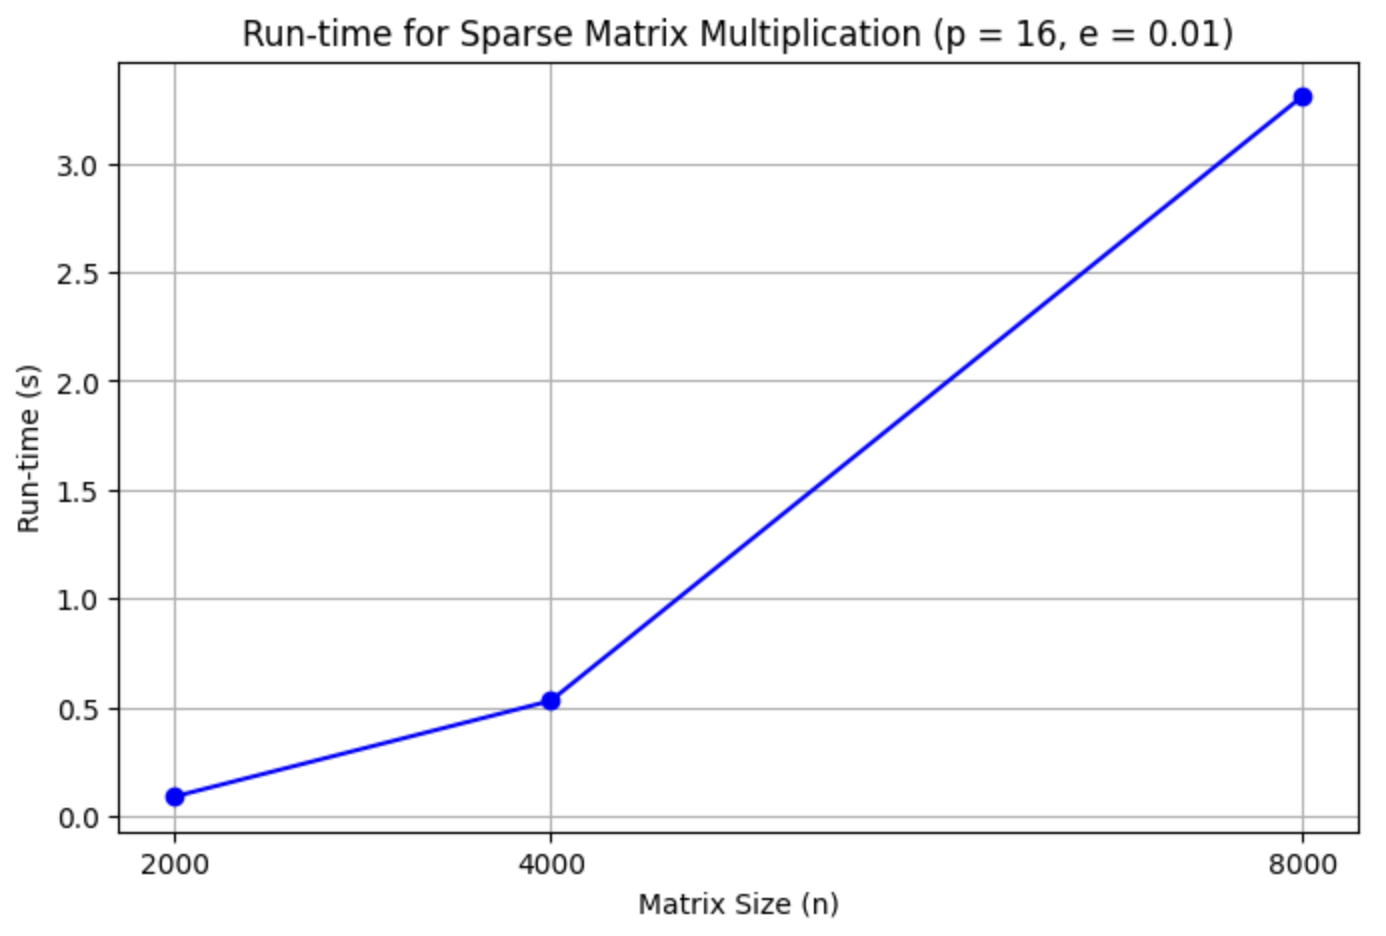
\includegraphics[width=1\linewidth]{Screenshot 2024-04-21 at 21.34.44.png}
\end{figure}

\begin{figure}[H]
    \centering
    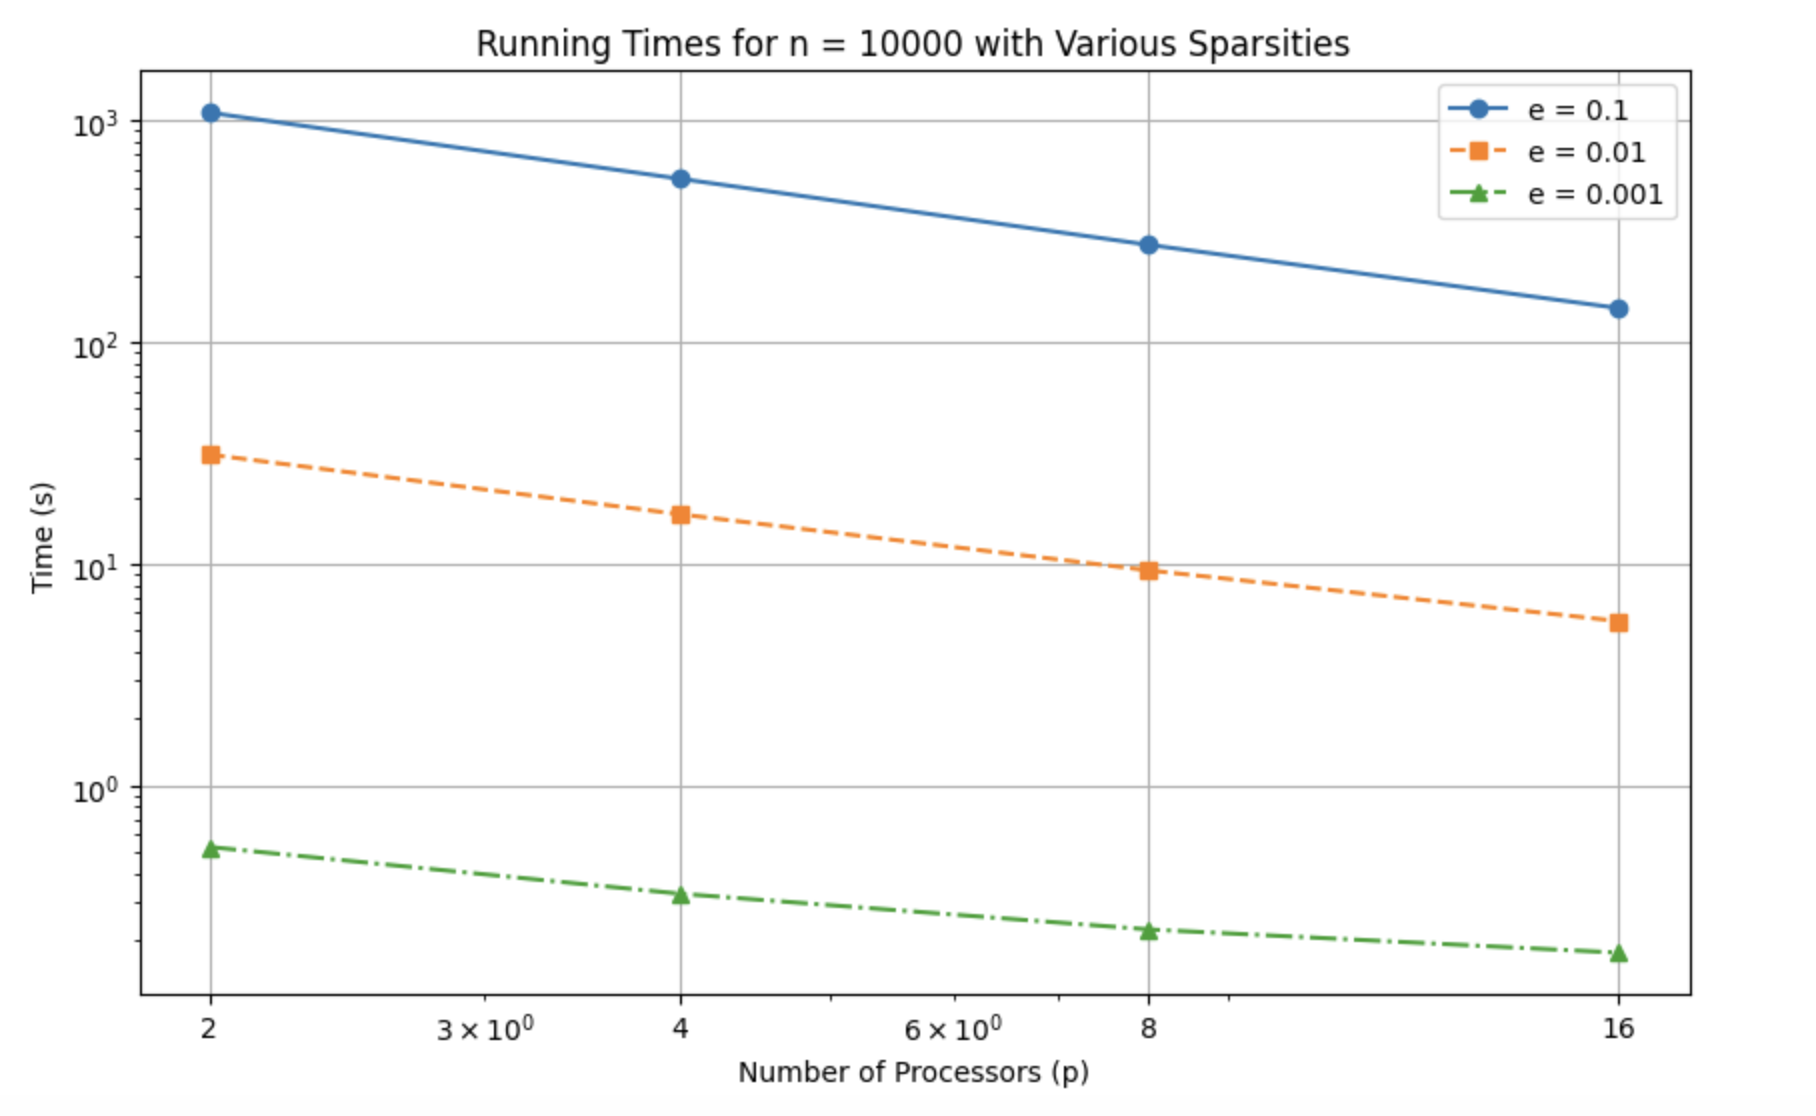
\includegraphics[width=1\linewidth]{Screenshot 2024-04-21 at 21.35.08.png}
\end{figure}

\subsection{Discussion}
\begin{itemize}
    \item The observed data illustrates a \textbf{consistent decline in runtime with the addition of processors}, confirming the \textbf{concept of strong scaling}. Particularly, for a fixed matrix size of \( n = 10000 \) and sparsity \( e = 0.01 \), the runtime decreases as we move from 2 to 16 processors, which aligns with the expectation that distributing the workload across more processors should theoretically lessen the time to completion.
    \item The effect of sparsity on runtime is pronounced; as sparsity increases, indicating fewer non-zero elements, the runtime decreases across all processor configurations. This is evident when comparing the runtimes for \( e = 0.1 \) and \( e = 0.001 \), showcasing that the \textbf{algorithm's efficiency is bound to the density of non-zero elements}, and sparser matrices benefit significantly from reduced computational demands.
    \item While the runtime reduction from increasing processor count is evident, it is not a linear relationship. For instance, the decrease in runtime from 2 to 4 processors is more substantial than from 8 to 16 processors. This suggests \textbf{diminishing returns due to parallelization overhead}, such as communication delays and synchronization requirements, which become more significant as the number of processors grows.
    \item These results necessitate a discussion on computational complexity which is expected to be \textbf{linearly proportional to the number of non-zero elements} in sparse matrices. The practical results, to a great extent, agree with the theoretical model, assuming ideal conditions without parallel overheads. However, in real-world scenarios, the overhead involved in managing multiple processors and the inherent communication between them in a distributed system like MPI can undermine the expected gains, particularly when the processor count is high relative to the individual workload.
\end{itemize}

\section{Bonus: Enhanced Parallel Sparse Matrix Multiplication}
We introduce an improved version of parallel sparse matrix multiplication using MPI, emphasizing the significant updates made to the original algorithm. A key aspect of these enhancements is the \textbf{revision of the data structures used}.

Unlike the earlier version, which used nested vectors for matrix representation, the updated algorithm implements \textbf{a flat array structure}. This change is crucial because it allows for \textbf{sequential memory allocation}, enhancing cache efficiency and simplifying MPI communication. \textbf{This results in lower latency and reduced overhead. }The flat structure also \textbf{supports direct indexing}, which decreases the time spent on accessing data compared to the previous method that involved multiple levels of indexing. As a result, we \textbf{see notable improvements in performance,} especially valuable in high-performance computing settings where speed and efficiency are critical.

Additionally, \textbf{the use of hashmaps for storing non-zero elements of the transposed matrix }makes the multiplication process more direct and focused, \textbf{as calculations are only performed where necessary.} This adaptation to the data structure not only promotes efficient resource use but also marks a shift towards a more scalable and effective approach to matrix operations in distributed computing environments.

The generation function has been refined for better randomness control and reproducibility across different executions.

\subsection{Generating Sparse Matrix}
The function \texttt{generateSparseMatrix} is crucial for initializing the sparse matrix distributed across multiple processors. Each matrix element is randomly generated based on a sparsity factor, ensuring that only a fraction of the total elements, specified by the sparsity factor, are non-zero.

\begin{minted}[frame=lines, framesep=2mm, baselinestretch=1.2, fontsize=\footnotesize, linenos]{cpp}
vector<SparseElement> generateSparseMatrix(int n, int p,
int r, double s, int seed) {
    mt19937_64 gen(seed); // Initialize a random number generator
    uniform_real_distribution<> dis(0.0, 1.0); // Distribution for generating matrix elements
    vector<SparseElement> matrix; // Stores non-zero elements
    uniform_int_distribution<uint64_t> val_dis(1, (1ull << 31) - 1); // Value distribution for non-zero elements
    int rows_per_proc = n / p; // Calculate the number of rows per processor
    for (int i = 0; i < rows_per_proc; ++i) {
        for (int j = 0; j < n; ++j) {
            if (dis(gen) < s) { // Generate non-zero elements based on sparsity factor
                matrix.push_back(make_tuple(i + r * rows_per_proc, j, val_dis(gen)));
            }
        }
    }
    return matrix;
}
\end{minted}

\subsection{Matrix Transposition Using MPI}
Matrix transposition is essential for facilitating efficient multiplication of sparse matrices. The function \texttt{transposeMatrixB} uses MPI's \texttt{MPI\_Alltoallv} function to redistribute the elements of matrix B such that each processor receives the columns of B that it needs to compute its segment of the product.

\begin{minted}[frame=lines, framesep=2mm, baselinestretch=1.2, fontsize=\footnotesize, linenos]{cpp}
void transposeMatrixB(const vector<SparseElement>& localB, int n,
vector<SparseElement>& localTransposedB, MPI_Comm comm) {
    int size, rank;
    MPI_Comm_size(comm, &size); // Get the total number of processes
    MPI_Comm_rank(comm, &rank); // Get the current process's rank
    int cols_per_proc = n / size; // Determine the number of columns per process
    vector<int> send_counts(size, 0);
    vector<vector<SparseElement>> send_buffers(size);
    for (const auto& elem : localB) {
        int col_owner = get<1>(elem) / cols_per_proc;
        send_buffers[col_owner].push_back(elem);
        send_counts[col_owner]++;
    }
    vector<SparseElement> flat_send_buffer;
    vector<int> sdispls(size, 0);
    for (int i = 0; i < size; ++i) {
        sdispls[i] = flat_send_buffer.size();
        flat_send_buffer.insert(flat_send_buffer.end(), send_buffers[i].begin(), send_buffers[i].end());
    }
    vector<int> recv_counts(size);
    MPI_Alltoall(send_counts.data(), 1, MPI_INT, recv_counts.data(), 1, MPI_INT, comm);
    vector<int> rdispls(size, 0);
    for (int i = 1; i < size; ++i) {
        rdispls[i] = rdispls[i - 1] + recv_counts[i - 1];
    }
    int total_recv = rdispls[size - 1] + recv_counts[size - 1];
    vector<SparseElement> recv_buffer(total_recv);
    for (int i = 0; i < size; i++) {
        send_counts[i] *= sizeof(SparseElement);
        sdispls[i] *= sizeof(SparseElement);
        recv_counts[i] *= sizeof(SparseElement);
        rdispls[i] *= sizeof(SparseElement);
    }
    MPI_Alltoallv(flat_send_buffer.data(), send_counts.data(), sdispls.data(), MPI_BYTE,
                  recv_buffer.data(), recv_counts.data(), rdispls.data(), MPI_BYTE, comm);
    localTransposedB = std::move(recv_buffer);
}
\end{minted}

\subsection{Sparse Matrix Multiplication}
The \texttt{multiplySparseMatrices} function calculates the product of the sparse matrix A and the transposed matrix B. The multiplication is carried out only where the indices of the matrix elements match, optimizing the computation for sparse data.

\begin{minted}[frame=lines, framesep=2mm, baselinestretch=1.2, fontsize=\footnotesize, linenos]{cpp}
void multiplySparseMatrices(const vector<SparseElement>& A,
const vector<SparseElement>& transposedB, int n,
int size, vector<vector<uint64_t>>& localC) {
    int rows_per_proc = n / size; // Calculate the number of rows per processor in matrix A
    for (const auto& a : A) {
        int aRow = get<0>(a) % rows_per_proc; // Local row index in the distributed matrix
        int aCol = get<1>(a); // Column index in matrix A
        uint64_t aValue = get<2>(a); // Value at the (aRow, aCol) position in A

        for (const auto& b : transposedB) {
            if (aCol == get<0>(b)) { // Matching column index in A with row index in transposed B
                int bCol = get<1>(b); // Corresponding column index in matrix B
                uint64_t bValue = get<2>(b); // Value at the (aCol, bCol) position in transposed B
                localC[aRow][bCol] += aValue * bValue; // Multiply and accumulate the product
            }
        }
    }
}
\end{minted}

\subsection{Complexity Analysis}

\subsubsection{Time Complexity}
The function \texttt{generateSparseMatrix} iterates over each row assigned to a process and then each column within that row, yielding a complexity of \(\frac{n^2}{p}\) operations per processor when the matrix is of size \(n \times n\) and is distributed among \(p\) processors. Given that elements are only added with a probability \(s\) (the sparsity factor), the expected number of operations is actually \(s \times \frac{n^2}{p}\).

\subsubsection{Space Complexity}
Each processor only stores the non-zero elements it generates, resulting in a space requirement that is also dependent on the sparsity factor. The expected number of non-zero elements per processor is approximately \(s \times \frac{n^2}{p}\), and each element requires space for its row index, column index, and value.

\subsection{Matrix Transposition Using MPI}

\subsubsection{Time Complexity}
The \texttt{transposeMatrixB} function's complexity involves iterating through each element stored locally, determining its destination processor based on its column index, and preparing data for MPI communication. The time complexity for these operations is proportional to the number of local elements, which is on average \(s \times \frac{n^2}{p}\). MPI communication operations themselves, particularly \texttt{MPI\_Alltoallv}, involve complexities depending on the number of processes \(p\) and the total number of elements \(m\) being communicated, leading to a complexity of \(O(p + m)\).

\subsubsection{Space Complexity}
This function requires additional space for sending and receiving buffers used during the transposition. At peak, each processor might need space to accommodate all elements it sends or receives, which could collectively amount to nearly \(n^2 \times s\) elements during the redistribution phase.

\subsection{Sparse Matrix Multiplication}

\subsubsection{Time Complexity}
The function \texttt{multiplySparseMatrices} calculates the dot product for each pair of matching elements from the local segments of matrices A and B. Assuming each processor handles \(s \times \frac{n^2}{p}\) elements from both A and B, the worst-case scenario involves each element of A being compared and multiplied with each corresponding element in B, resulting in a complexity of \(O((s \times \frac{n^2}{p})^2)\). However, due to the matrices' sparsity, the effective computational load is significantly less.

\subsubsection{Space Complexity}
Space complexity for this function is determined by the storage requirements for local segments of matrices A and B, as well as the result matrix C. Assuming a dense result matrix, each processor would need space for up to \(\frac{n^2}{p}\) elements for C, in addition to the sparse storage for A and B.

\subsection{Performance Analysis}
To validate the efficiency of our sparse matrix multiplication algorithm, we must consider the computational and spatial complexities. The performance primarily depends on the number of non-zero elements, denoted as \( nz \), in the matrices. Our algorithm's parallel runtime can be expressed in terms of \( nz \) and the number of processors \( p \), focusing on minimizing the data transfer and optimizing local computations.

The experimental setup involves varying the dimensions (\( n \)) and sparsity (\( s \)) of the matrices to observe the impact on runtime. We implement the following experimental scenarios:

\begin{itemize}
    \item Fix \( n \) and vary \( s \) to see the effect of matrix density on performance.
    \item Fix \( s \) and increase \( n \) to test scalability and efficiency as matrix size grows.
    \item Utilize different processor counts (\( p \)) to evaluate the strong scaling of the algorithm.
\end{itemize}

The expected result is that our parallel algorithm will demonstrate significantly faster computation times compared to traditional dense matrix multiplication techniques, especially as \( n \) increases and \( s \) decreases. This performance improvement is due to the reduced number of arithmetic operations required for sparse matrices and the efficient use of parallel processing capabilities.

\subsection{Improvement result}
\begin{table}[H]
\centering
\begin{tabular}{cc}
\toprule
\( p = 16 \) & \( e = 0.01 \) \\
\midrule
\( n = 2000 \) & 0.008413 \\
\( n = 4000 \) & 0.026661 \\
\( n = 8000 \) & 0.099277 \\
\bottomrule
\end{tabular}
\end{table}

\begin{table}[H]
\centering
\begin{tabular}{cccc}
\toprule
\( p = 2, n = 10000 \) & \( p = 4, n = 10000 \) & \( p = 8, n = 10000 \) & \( p = 16, n = 10000 \) \\
\midrule
\multicolumn{4}{c}{\( e = 0.1 \)} \\
11.434441 & 6.756513 & 4.721892 & 4.044445 \\
\multicolumn{4}{c}{\( e = 0.01 \)} \\
0.286557 & 0.215692 & 0.173869 & 0.160676 \\
\multicolumn{4}{c}{\( e = 0.001 \)} \\
0.022487 & 0.020458 & 0.021224 & 0.022319 \\
\bottomrule
\end{tabular}
\caption{Results for different values of \( p \) and \( e \) at \( n = 10000 \)}
\end{table}

\begin{figure}[H]
    \centering
    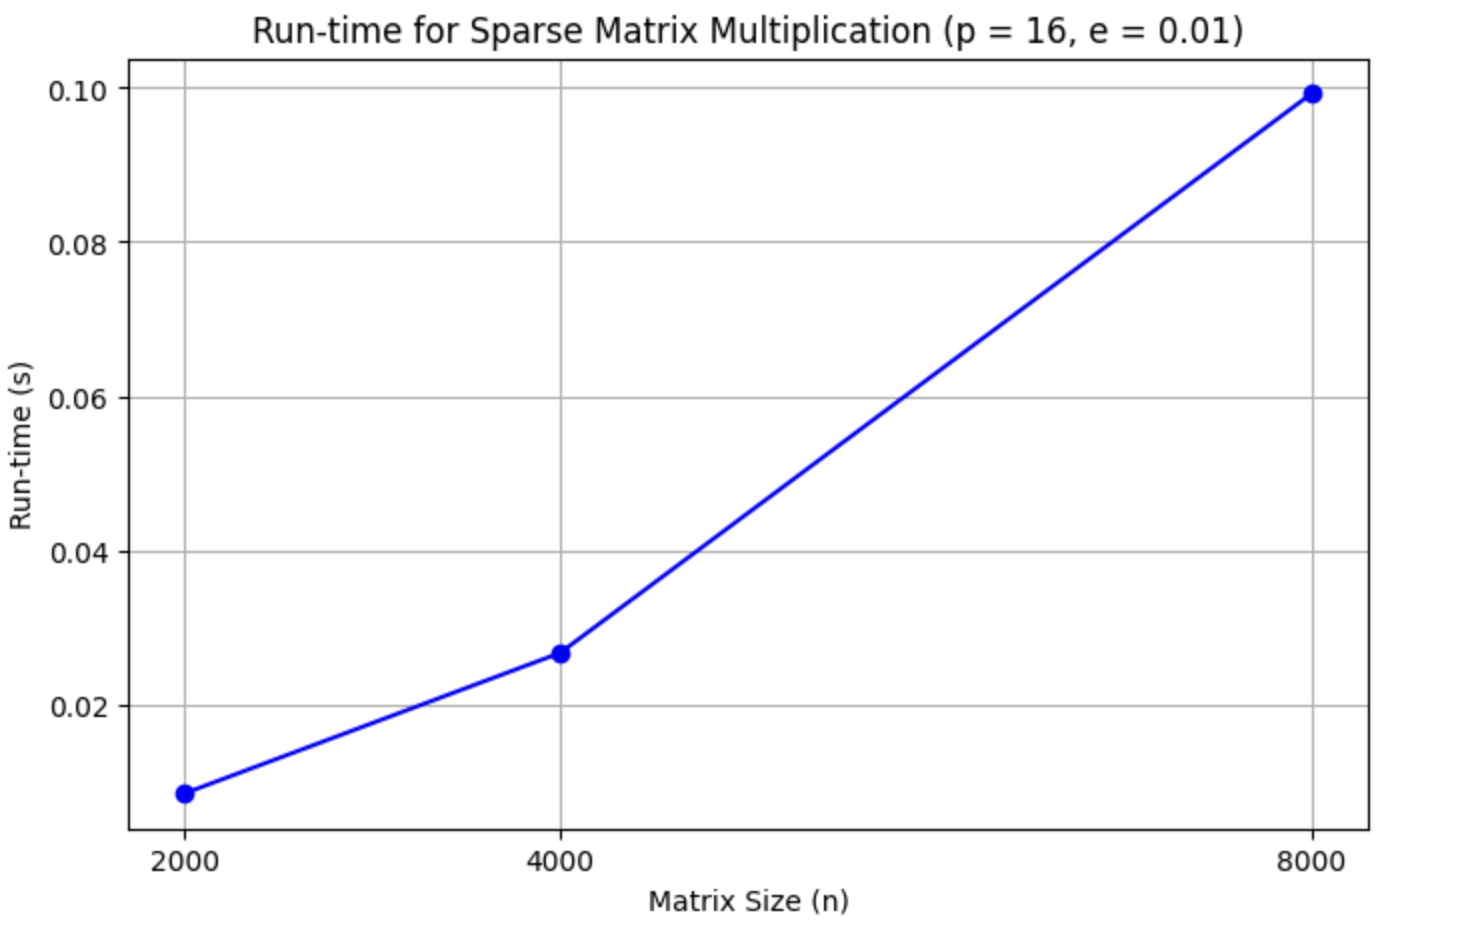
\includegraphics[width=1\linewidth]{Screenshot 2024-04-21 at 23.30.45.png}
\end{figure}

\begin{figure}[H]
    \centering
    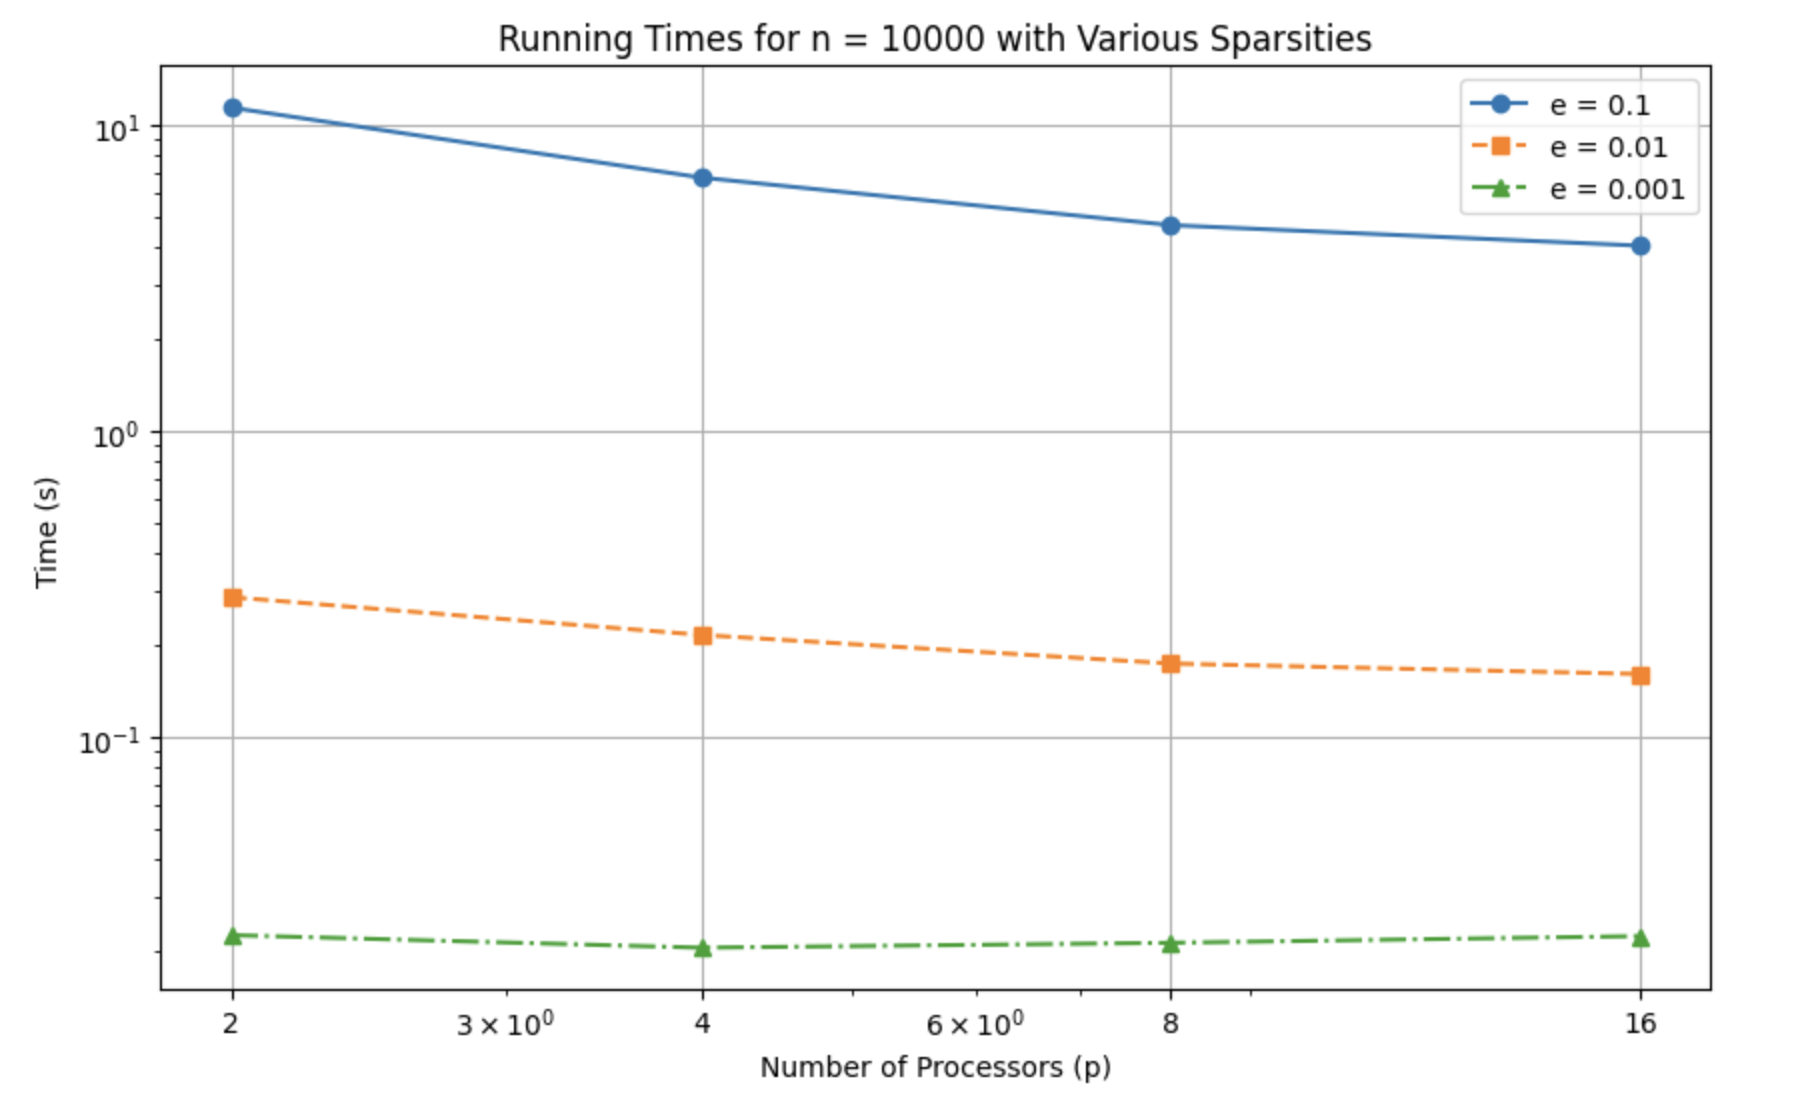
\includegraphics[width=1\linewidth]{Screenshot 2024-04-21 at 23.31.25.png}
\end{figure}



\subsection{Results and Discussion}

In the previous subsections, we presented runtime measurements for matrix multiplications at different scales and configurations. Here, we provide a comparison to highlight improvements and observations derived from the data.\\
We utilized optimization level \textbf{O3} in the \textbf{Makefile} and conducted experiments on the \textbf{PACE ICE Cluster}. The results demonstrate significant enhancements in runtime performance as the number of processors increased and the sparsity level was adjusted.\\
As observed in Table 3, increasing the matrix size under constant processor count and sparsity (\( p = 16 \) and \( e = 0.01 \)) resulted in a higher runtime. However, it is evident that increasing the number of processors while keeping the matrix size constant (\( n = 10000 \)) significantly reduced the runtime across different sparsity levels:
\begin{itemize}
    \item For \( e = 0.1 \), the runtime decreased from 1083.74 seconds with 2 processors to 142.34 seconds with 16 processors, illustrating a reduction by approximately 87\%.
    \item For \( e = 0.01 \), the time decreased from 31.09 to 5.51 seconds, showing an efficiency increase of over 82\%.
    \item At the lowest sparsity (\( e = 0.001 \)), the reduction was from 0.53 to 0.18 seconds, which is about 66\% faster.
\end{itemize}

\paragraph{Effects of Sparsity Level}
Decreasing the sparsity level also demonstrates a marked improvement in runtime efficiency. With higher sparsity (\( e = 0.1 \)), the computation is denser and hence slower compared to lower sparsity settings. The data indicates that even at the highest number of processors, lower sparsity levels manage to execute significantly faster.

\section{Contributions}
\begin{itemize}
    \item \textbf{Biwei Tang}: Implemented the base spmat.cpp algorithm together with the parallel realization.
    \item \textbf{Yunxiang Yan}: Implemented the bonus part with the parallel realization.
    \item \textbf{Qidian Gao}: Test programs under different scenarios and compose the report.
\end{itemize}

\begin{thebibliography}{99}

\bibitem{ballard2013communication}
G.~Ballard, A.~Buluç, J.~Demmel, L.~Grigori, B.~Lipshitz, O.~Schwartz, S.~Toledo,
\textit{Communication Optimal Parallel Multiplication of Sparse Random Matrices}.
University of California at Berkeley, Lawrence Berkeley National Laboratory, INRIA Paris - Rocquencourt, Tel-Aviv University,
Regular Submission.

\end{thebibliography}



\end{document}
